\documentclass{article}

\usepackage[utf8]{inputenc}
\usepackage[style=phys]{biblatex}
\usepackage{graphicx}

\bibliography{refs}

\begin{document}
  \begin{flushright}
    Zach Colbert \\
    Thesis - PH 403 \\
    27 Nov 2018 \\
  \end{flushright}

  \begin{center}
    \textbf{Primary Literature Assignment} \\
  \end{center}

  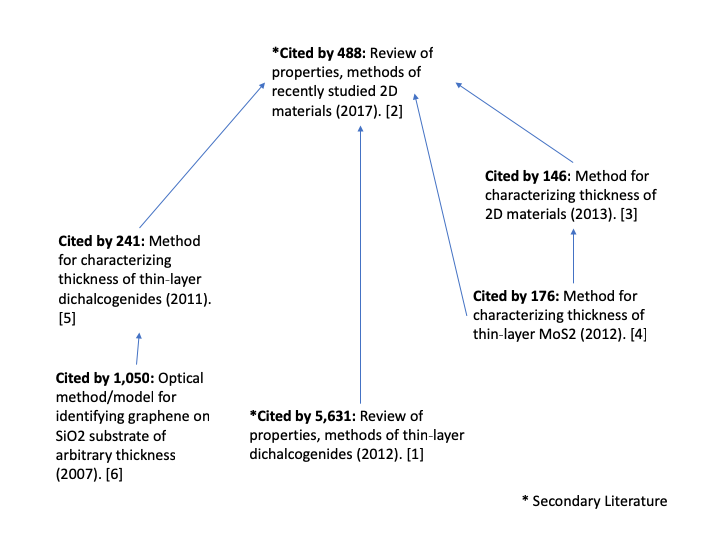
\includegraphics[width=\textwidth]{map.png}

  I actually started by finding Wang's paper \cite{wang_electronics_2012} in a Google Scholar search. It is not primary literature, but a review of many works in the field--this made it a nice starting place. By pulling up this paper on Web of Science, I was able to look at a list of papers that cited this one and found a similar, more recent paper from Tan \cite{tan_recent_2017}. \par

  Because Tan is a long review of many other works, it is rich with citations. The paper covers broad topics surrounding materials that my group works with, so I went looking in the table of contents for optical and electronic methods that might be related to my work. Reading through sections on imaging these materials, I found some interesting method papers from Li \cite{li_optical_2012,li_rapid_2013} and Benameur \cite{benameur_visibility_2011}. These papers are primary literature because they directly report the development and results of an experiment, and are published in peer-reviewed journals. \par

  Looking through the references in Benameur, I found a lot of books and what seemed to be secondary literature. I did, however, find an interesting piece of primary literature from Blake \cite{blake_making_2007}, that describes an earlier method used to characterize graphene specifically, which seems to have led to the broader application used by Benameur.

  \newpage

  \printbibliography
\end{document}